% Forrás: Fleiner Tamás gyakorlat

\documentclass[tikz]{standalone}
\usepackage{tikz}
\usetikzlibrary{positioning, graphs}
\usetikzlibrary{graphs.standard}
\begin{document}
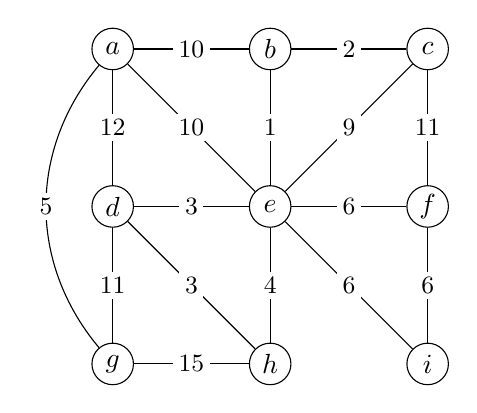
\begin{tikzpicture}
		[vertex/.style={draw,circle,inner sep = 0mm, minimum size = 15},
         edgelabel/.style = {fill = white, inner sep = 2, font=\small}]

        \node[vertex] (a) at (0,  4) {$a$};
        \node[vertex] (b) at (2, 4) {$b$};
        \node[vertex] (c) at (4, 4) {$c$};
        \node[vertex] (d) at (0, 2) {$d$};
        \node[vertex] (e) at (2, 2) {$e$};
        \node[vertex] (f) at (4, 2) {$f$};
        \node[vertex] (g) at (0, 0) {$g$};
        \node[vertex] (h) at (2, 0) {$h$};
        \node[vertex] (i) at (4, 0) {$i$};

        \draw[-] (a) to node[edgelabel] {$10$} (b);
        \draw[-] (a) to node[edgelabel] {$12$} (d);
        \draw[-] (a) to node[edgelabel] {$10$} (e);
        \draw[-] (a) to [bend right=40] node[edgelabel] {$5$} (g);
        \draw[-] (b) to node[edgelabel] {$2$} (c);
        \draw[-] (b) to node[edgelabel] {$1$} (e);
        \draw[-] (c) to node[edgelabel] {$9$} (e);
        \draw[-] (c) to node[edgelabel] {$11$} (f);
        \draw[-] (d) to node[edgelabel] {$3$} (e);
        \draw[-] (d) to node[edgelabel] {$11$} (g);
        \draw[-] (d) to node[edgelabel] {$3$} (h);
        \draw[-] (e) to node[edgelabel] {$6$} (f);
        \draw[-] (e) to node[edgelabel] {$4$} (h);
        \draw[-] (e) to node[edgelabel] {$6$} (i);
        \draw[-] (f) to node[edgelabel] {$6$} (i);
        \draw[-] (g) to node[edgelabel] {$15$} (h);
		
\end{tikzpicture}
\end{document}